\chapter{投影光学与结构光}
\label{ch:06}

\section{效果}
\label{sec:ch06-effect}

读完本章，你应能：
\begin{enumerate}
  \item 把投影仪看作「倒装的相机」，说明其光路、景深与畸变如何进入结构光几何；
  \item 写出正弦条纹模型与 $N$ 步相移求相位 $\varphi$ 的公式，并给出调制度、$\SNR$ 与相位噪声的关系；
  \item 用时间相位展开、多频外差与格雷码的直觉解释「包裹相位如何变成绝对相位」，以及各自的失效方式；
  \item 叙述从绝对相位到深度 $(X,Y,Z)$ 的标定链；
  \item 说明 DMD 与 LCoS 的调制概念：二值调制、离焦成正弦、伽马非线性、帧同步；
  \item 诊断口内结构光中的高反、次表面散射与运动伪影。
\end{enumerate}

\section{原理}
\label{sec:ch06-principle}

\subsection{投影仪：倒装的相机}

投影仪由光源、匀光、空间光调制器（DMD 或 LCoS 等）与投影镜头组成。几何上，它与相机互为对偶：相机把空间射线映到像素 $(u,v)$；投影仪把调制器像素 $(u_p,v_p)$ 映为空间射线。因此投影仪同样有内参 $K_p$、畸变与外参，第~\ref{ch:02}~章的模型可原样搬用，只是「像面」换成调制器平面。

投影镜头的景深同样有限。条纹投到工作距范围之外时，投影侧离焦先把条纹模糊，相机侧离焦再模糊一次；两次 $\PSF$ 的卷积共同决定相机所见调制度。口内设备常让投影与相机共用或靠近同一工作距，并选较小相对孔径以换取景深 $Z_d$，代价是光通量（第~\ref{ch:05}~章）。

\subsection{正弦条纹模型}

投影仪沿一个方向（设为 $u_p$）投出周期为 $P$ 像素的正弦条纹。物体表面反射后，相机像素 $(u,v)$ 处的第 $k$ 帧灰度可写作
\begin{equation}
  I_k(u,v)=A(u,v)+M(u,v)\cos\!\bigl(\varphi(u,v)+\delta_k\bigr),\qquad k=0,\dots,N-1,
  \label{eq:ch06-fringe}
\end{equation}
其中 $A$ 为背景（含环境光与平均反射），$M$ 为调制幅度，$\delta_k$ 为第 $k$ 帧的已知相移，$\varphi$ 为待求相位。$\varphi$ 编码了「该相机像素看到的是投影仪哪一列」：$u_p=\dfrac{P}{2\pi}\varphi$。这里的强度沿用相对强度 $I$，前提是相机工作在线性区且曝光锁定（第~\ref{ch:05}~章）。

相机所见的调制度（条纹对比度）记为 $V=M/A$，与第~\ref{ch:03}~章的可见度是同一个量；投影端（调制器上）的调制度记为 $V_0$。离焦、次表面散射、环境光都会降低 $V$。

\subsection{$N$ 步相移}

取等间隔相移 $\delta_k=2\pi k/N$（$N\ge3$）。最小二乘解为
\begin{equation}
  \varphi_w=\operatorname{atan2}\Bigl(-\sum_{k}I_k\sin\delta_k,\ \sum_{k}I_k\cos\delta_k\Bigr),
  \label{eq:ch06-nstep}
\end{equation}
\begin{equation}
  M=\frac{2}{N}\sqrt{\Bigl(\sum_k I_k\sin\delta_k\Bigr)^2+\Bigl(\sum_k I_k\cos\delta_k\Bigr)^2},
  \qquad
  A=\frac{1}{N}\sum_k I_k.
  \label{eq:ch06-AM}
\end{equation}
四步（$N=4$）时简化为
\[
  \varphi_w=\operatorname{atan2}(I_3-I_1,\ I_0-I_2).
\]
所得 $\varphi_w$ 落在 $(-\pi,\pi]$，称为包裹相位（图~\ref{fig:ch06-fringe}）。

\textbf{相位噪声。} 若每帧灰度噪声标准差为 $\sigma_I$（加性、独立），相位标准差约为
\begin{equation}
  \sigma_{\varphi}\approx\sqrt{\frac{2}{N}}\,\frac{\sigma_I}{M}.
  \label{eq:ch06-phase-noise}
\end{equation}
即相位精度正比于「调制幅度对噪声」的比，而不是「平均亮度对噪声」。$M$ 小而 $A$ 大（环境光强、散射严重）时，光子噪声随 $A$ 增长而 $M$ 不长，相位反而更差。这是结构光的 $\SNR$ 应定义在调制项上的原因。增大 $N$ 以 $\sqrt{N}$ 降噪，但需要更多帧，对运动更敏感。

$N$ 步相移还有一个好处：若相机或投影存在伽马非线性，谐波会引入周期性相位误差；$N$ 越大，越高阶的谐波才会混叠进相位，因此误差越小。

\begin{figure}[htbp]
  \centering
  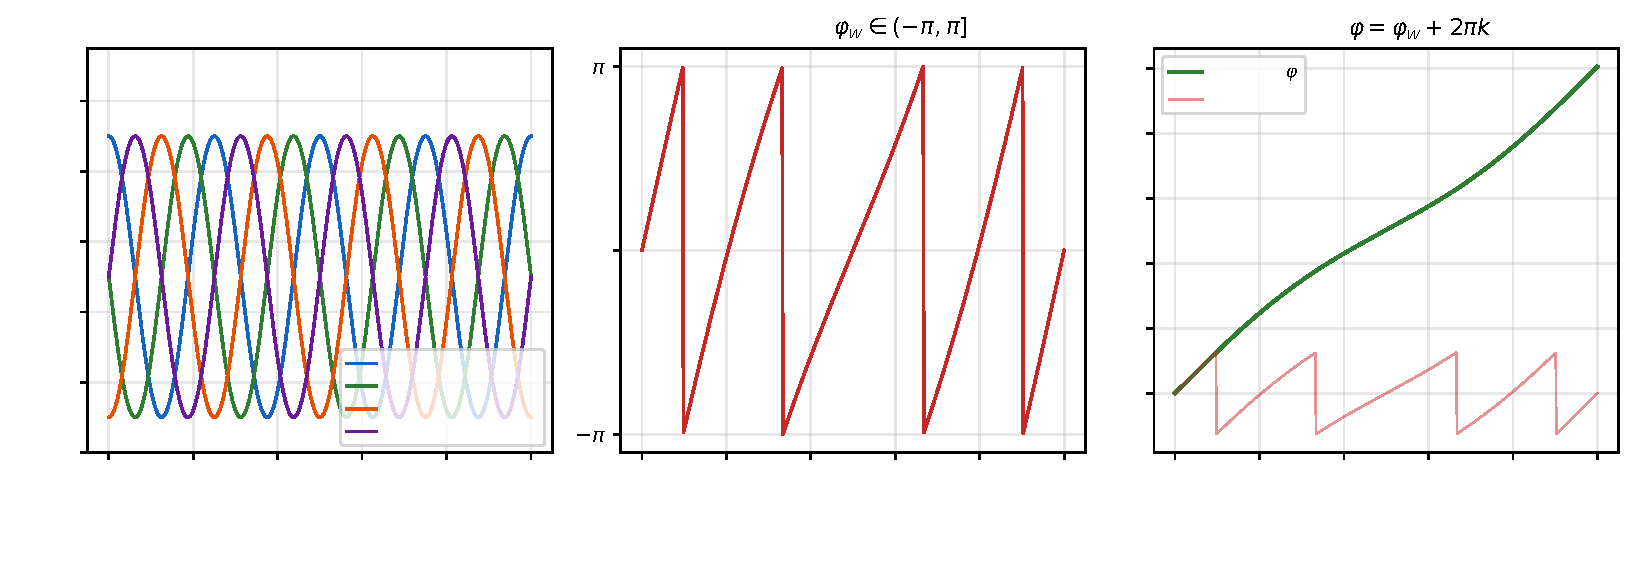
\includegraphics[width=0.98\textwidth]{fig-fringe-phase.pdf}
  \caption{四步相移条纹截面、包裹相位与展开相位的概念草图（非精确工程图）。}
  \label{fig:ch06-fringe}
\end{figure}

\subsection{相位展开}

包裹相位只给出「在一个条纹周期内的位置」，还需确定整数级次 $k$：$\varphi=\varphi_w+2\pi k$。两类思路：

\textbf{空间展开。} 沿图像路径累加相邻像素的相位差，假设相邻像素差不超过 $\pi$。在连续光滑表面有效；遇到遮挡、陡坡、孤立区域（牙间隙、器械边缘）时会把错误传播开来。质量引导、最小范数等方法改进了鲁棒性，系统论述见 \citet{GhigliaPritt1998}。

\textbf{时间展开。} 每个像素独立地用额外图案确定 $k$，不依赖邻域，因此对不连续表面更稳。常见三种：
\begin{itemize}
  \item \textbf{多频（外差）}：投两个或多个周期 $P_1<P_2$ 的条纹，其相位差相当于等效长周期 $P_{\mathrm{eq}}=P_1P_2/(P_2-P_1)$。等效周期覆盖整个视场时，即可逐级确定高频条纹的级次。代价是噪声在逐级推导中被放大 $P_{\mathrm{eq}}/P_1$ 倍，频率比不能选得过大。
  \item \textbf{格雷码}：投 $m$ 幅二值图案，给每个条纹周期编号 $0,\dots,2^m-1$。格雷码相邻编号只差一位，边界上误判最多错一级。弱点是黑白边界处被模糊后易判错，常出现「级次跳变一个周期」的线状误差，需要与包裹相位边界对齐校正。
  \item \textbf{相位编码 / 其他}：把级次编码在额外的相位图中，原理相近。
\end{itemize}
共同点：高频条纹负责精度，低频或编码负责唯一性。设计时先让最高频条纹在工作距内仍有足够 $M$（第~\ref{ch:03}~章的通带），再选最少的辅助图案保证展开正确。

\subsection{从相位到深度：标定链}

绝对相位 $\varphi$ 给出投影仪列坐标 $u_p$。与相机像素 $(u,v)$ 一起，就有一对对应：相机射线与投影仪的一张「光平面」（单方向条纹时是平面，而非射线）。三角求交即得 $(X,Y,Z)$。所需参数：
\begin{enumerate}
  \item 相机内参 $K$ 与畸变；
  \item 投影仪内参 $K_p$ 与畸变（通常借助相机「替投影仪看」标定板：投影仪通过相位反算标定板角点的 $(u_p,v_p)$）；
  \item 两者相对外参 $R,t$。
\end{enumerate}
另一种做法是\textbf{相位–高度查表}：在若干已知高度的平面上记录每像素的相位，拟合 $Z=g_{uv}(\varphi)$ 多项式。查表绕开显式模型，对投影畸变不敏感，但只在标定过的深度范围内可靠，外推会出错。

两种方法都要求：标定时与工作时的曝光、对焦、伽马处理、投影亮度完全一致；任何改变都会使 $\varphi$ 到 $Z$ 的映射漂移。

\subsection{DMD 与 LCoS：调制概念}

\textbf{DMD（数字微镜器件）} 由大量可在两种倾角间翻转的微镜组成。「开」镜把光反射进投影镜头，「关」镜反射到吸收器。单个微镜只能二值；灰度靠在一帧内按比特面控制开关时间（脉宽调制）。这带来两个工程后果：
\begin{itemize}
  \item 相机曝光若不是比特周期的整数倍，或未与投影帧同步，会截取到不完整的比特序列，灰度出错，表现为条纹「跳灰度」或帧间闪烁；
  \item 灰度正弦需要多个比特面，帧率下降。
\end{itemize}

\textbf{二值离焦法}：直接投二值方波条纹，让投影镜头适度离焦，方波高次谐波被 $\MTF$ 衰减，到达物体时近似正弦（图~\ref{fig:ch06-dmd}）。优点：一个比特面一帧，可上千赫兹，并且没有伽马问题。缺点：近似正弦的程度依赖离焦量，即依赖深度；残余谐波造成周期性相位误差。

\textbf{LCoS（硅基液晶）} 通过液晶对偏振态的调制实现连续灰度，需要偏振光照明与检偏（第~\ref{ch:04}~章），响应较慢，有灰度–电压非线性。

\textbf{伽马。} 投影仪与相机的灰度响应常非线性，投入的「正弦」实际变成含谐波的周期曲线，导致相位误差呈条纹周期的 $N$ 倍频波纹。对策：标定伽马曲线并预失真；或增加相移步数；或使用二值离焦。

\begin{figure}[htbp]
  \centering
  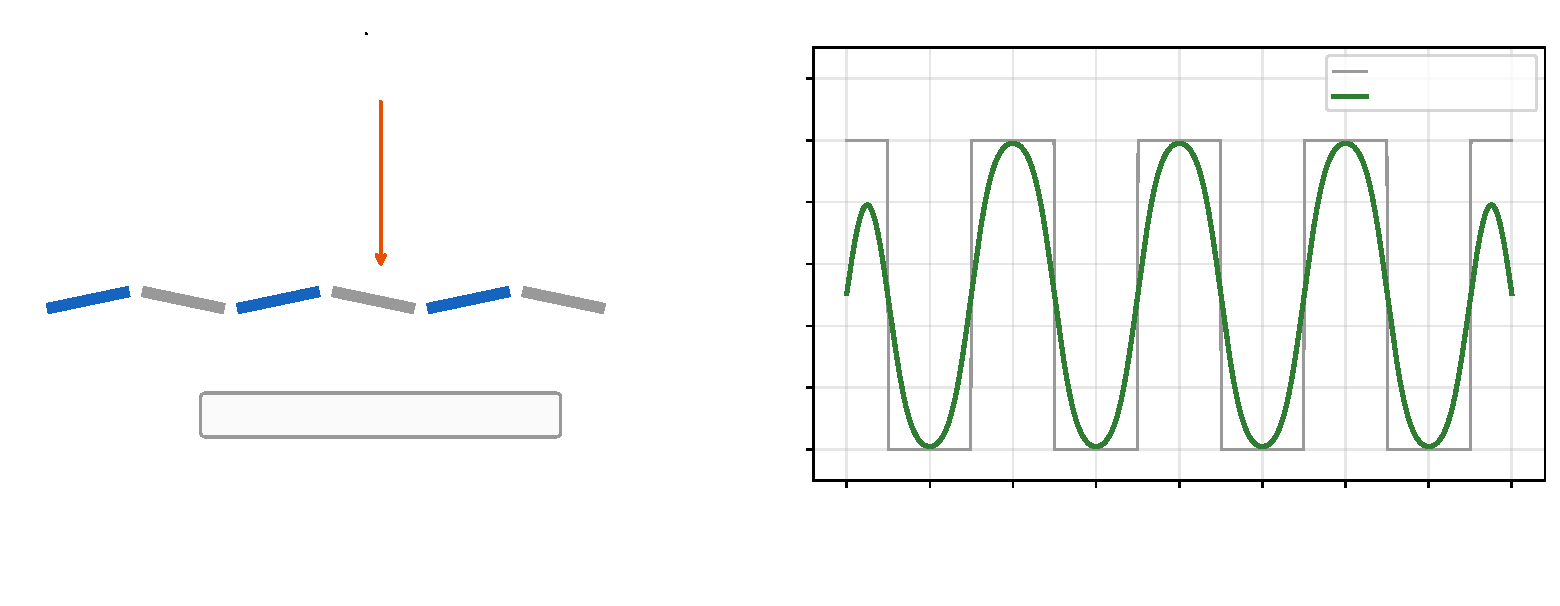
\includegraphics[width=0.95\textwidth]{fig-dmd-concept.pdf}
  \caption{DMD 微镜二值开关与二值条纹经离焦近似为正弦的概念草图（非精确工程图）。}
  \label{fig:ch06-dmd}
\end{figure}

\section{限度}
\label{sec:ch06-limits}

\begin{itemize}
  \item 式~\eqref{eq:ch06-fringe} 假设每像素只接收来自投影仪一个位置的直接反射。次表面散射与互反射违反该假设，属于模型误差，不是噪声。
  \item 式~\eqref{eq:ch06-phase-noise} 假设加性独立噪声与静止物体；运动与非线性误差需要另外计算。
  \item 多频与格雷码展开都假设辅助图案在工作距内可辨；景深外首先失效的往往是展开，而不是包裹相位本身。
  \item 相位–高度查表只对标定范围内深度有效。
  \item 本章不涉及单帧方法（傅里叶变换轮廓术、彩色编码、学习方法）的完整推导；它们以空间带宽或颜色换时间，仍受同样的光学限制。
\end{itemize}

\section{对象}
\label{sec:ch06-object}

\textbf{口内结构光。} 工作距约十余毫米，景深仅数毫米，探头手持移动。常见折中：中高频条纹 + 少帧相移 + 时间展开，配合高帧率投影与全局快门相机。每多一帧，运动伪影风险就增加一份；每少一帧，相位噪声与伽马误差就增加一份。

\textbf{高反（釉质湿润面、金属修复体）。} 高光处相机饱和，式~\eqref{eq:ch06-fringe} 削顶，相位错误且 $M$ 计算值异常。诊断：检查 $I_k$ 是否触顶；用 $M$ 与 $A$ 做质量图并掩膜。对策：交叉偏振、多曝光合成（锁定每档曝光，不用自动曝光）、喷粉（临床上逐渐被避免）。

\textbf{次表面散射（牙本质、牙龈、半透明修复材料）。} 光进入材料后在内部扩散再射出，相当于条纹被一个空间核模糊并平移。结果：调制度 $M$ 下降、相位偏移，深度出现系统性的「下沉」或「平滑」。中低频条纹下，散射核宽度小于周期，散射光仍带着被平移的条纹，造成相位偏置；当条纹周期明显短于散射核宽度时，散射光被平均成近似常数，进入 $A$ 而不再偏置 $\varphi$，代价是 $M$ 降低。对策因此是：在 $M$ 仍够用的前提下提高条纹频率；短波长（蓝光）穿透更浅，常用于口内。

\textbf{运动伪影。} $N$ 帧之间物体移动 $\Delta u$ 像素，相当于每帧的 $\varphi$ 不同，求解得到的相位有与条纹同周期的波纹误差。诊断：静止模型上误差消失；误差随移动速度增大。对策：缩短总采集时间（提高投影帧率、减少帧数）、运动补偿、或用对运动不敏感的编码顺序。

\section*{本章收束}
结构光把「投影仪哪一列照到这里」编码为相位 $\varphi$。相移决定相位精度，展开决定唯一性，标定决定相位到深度的映射。DMD 与 LCoS 的调制方式决定伽马、同步与帧率。对象场景中的误差大多可归入：调制度不足、模型假设被违背（散射、饱和）、帧间不一致（运动、曝光）。下一章讨论三角测量本身如何放大这些误差。

\section{习题}
\label{sec:ch06-exercises}

\begin{enumerate}
  \item \textbf{（计算）} 四步相移得到 $I_0=180,\ I_1=100,\ I_2=60,\ I_3=140$。求包裹相位 $\varphi_w$、$A$、$M$ 与调制度 $M/A$。
  \item \textbf{（计算）} 三步与六步相移，若 $\sigma_I/M$ 相同，相位标准差之比是多少？六步的代价是什么？
  \item \textbf{（计算）} 两组条纹周期 $P_1=16$ 像素、$P_2=18$ 像素。求等效周期 $P_{\mathrm{eq}}$。若投影仪宽 $912$ 像素，等效周期能否覆盖全宽？噪声放大倍数约为多少？
  \item \textbf{（重建场景）} 某口内扫描点云在牙龈与半透明修复体上比釉质「低」约几十微米，且条纹频率提高后差异减小。解释原因。
  \item \textbf{（重建场景）} 点云上出现沿条纹方向、间距恰为一个条纹周期深度的线状台阶。最可能是哪一步出错？如何确认？
  \item \textbf{（重建场景）} 相位误差图出现频率为条纹频率 $4$ 倍的规则波纹（四步相移）。可能原因是什么？给出两种对策。
  \item \textbf{（设计）} DMD 投影帧率 $1000$ 帧/秒（二值），相机全局快门。设计一个「二值离焦 + 时间展开」的采集序列，估计总时长，并说明手持速度 $20\,\mathrm{mm/s}$ 时的运动量。
\end{enumerate}

\section{习题讲解}
\label{sec:ch06-solutions}

\begin{enumerate}
  \item $\varphi_w=\operatorname{atan2}(I_3-I_1,\,I_0-I_2)=\operatorname{atan2}(40,120)\approx0.32\,\mathrm{rad}$。$A=(180+100+60+140)/4=120$。$M=\tfrac12\sqrt{40^2+120^2}\approx63.2$。调制度 $M/A\approx0.53$。
  \item $\sigma_\varphi\propto\sqrt{2/N}$，三步比六步为 $\sqrt{6/3}=\sqrt2\approx1.41$。六步需双倍时间，运动更敏感，帧率更低。
  \item $P_{\mathrm{eq}}=16\times18/(18-16)=144$ 像素，不足以覆盖 $912$ 像素，需要第三个频率或格雷码辅助。噪声放大约 $P_{\mathrm{eq}}/P_1=9$ 倍，因此级次判定要求低频相位噪声小于约 $\pi/9$。
  \item 次表面散射：光在半透明材料内扩散，条纹被模糊并偏移，相位偏置使深度系统性偏差。提高条纹频率使散射成分更接近常数背景，偏置减小。
  \item 相位展开级次错一级（格雷码边界误判或多频级次误判）。确认：在包裹相位图上看台阶是否位于 $\pm\pi$ 跳变处；检查格雷码解码在边界上是否与包裹相位不同步。
  \item 伽马非线性（投影或相机），也可能是 DMD 未同步导致的灰度误差。对策：伽马标定与预失真；增加相移步数；改二值离焦；检查帧同步。
  \item 例：$3$ 幅格雷码或 $2$ 组低频 + $4$ 步高频相移，约 $7$--$12$ 帧，$7$--$12\,\mathrm{ms}$。移动 $0.14$--$0.24\,\mathrm{mm}$，相对于数十微米的精度目标很大，需要缩短序列或做运动补偿。
\end{enumerate}
